\documentclass[12pt,a4paper,final,oneside,openright,onecolumn,titlepage]{scrbook}

\usepackage[utf8]{inputenc}
\usepackage{csquotes}
%\usepackage[english]{babel}
\usepackage{dirtytalk}
\usepackage{graphicx}
\usepackage{titling}
%\usepackage{fontspec}
%\setmainfont[Ligatures=TeX]{Bitter-Regular.ttf}
%\usepackage[left=2.cm,right=3cm,top=2cm,bottom=2cm]{geometry}
\usepackage[style=authoryear,maxcitenames=2, backend=biber,showmedium=true,useprefix=false]{biblatex}
\usepackage{acronym}
%\usepackage[T1]{fontenc}
\usepackage{titlesec, blindtext, color}
\usepackage{float}
\usepackage{subcaption}
\usepackage{cleveref}
\usepackage{array}
%\usepackage{wrapfig}

\newcommand{\sekcite}[4]{%
(\cite[#2]{#1} qtd.\ in \cite[#4]{#3})%
}

\newcounter{savepage}

\renewcommand{\baselinestretch}{1.5}
\titleformat{\chapter}[hang]{\Huge\bfseries}{\thechapter \hspace{20pt} }{0pt}{\Huge\bfseries}

\newcommand{\ssay}[1]{%
    \mbox{\say{#1}}%
}

\bibliography{bibliography}

\author{Nick London}

\title{Conceptual Aspects of Mobile Applications regarding Customer Purchasing Behaviour in a Business-to-Business Context}

\clubpenalty = 10000 
\widowpenalty = 10000 
\displaywidowpenalty = 10000

\begin{document}
\begin{titlepage}
	\includegraphics[height=8em]{img/logos/dhbw.pdf}
	\hfill
	\raisebox{3.5em}{
\includegraphics[height=3em]{img/logos/ibm.pdf}}\par
	\centering
	\vfill
	{\huge \textsc{\MakeUppercase{Bachelorthesis}}\par}
	\vspace{2em}
	{\Huge \textbf{\thetitle}\par}
	\vspace{1.5em}
	{\large Nick~\textsc{London}\par}
	\vfill
	{\small IBM~Deutschland~MBS~GmbH\par
	International~Management~for~Business~and~Information~Technology\par
	Matriculation~Number:~7203669}
	\vfill
	{scientifically supervised by\par Prof.~Dr.~Rainer~\textsc{Beedgen}\par}
	\par\vspace{1em}
	{practically supported by\par ~Markus \textsc{Sachs}\par}
	\vspace{2em}
	{Time allowed for completion\par April 11, 2017 to July 04, 2017\par}
\end{titlepage}

\pagenumbering{Roman}
\setcounter{page}{1}

\addcontentsline{toc}{section}{Contents}
\tableofcontents

\newpage
\addcontentsline{toc}{section}{List of Figures}
\listoffigures

\newpage
\addcontentsline{toc}{section}{List of Tables}
\listoftables

\pagebreak
% Abkürzungsverzeichnis 
\chapter*{Abbreviations} %Bitte alphabetisch ordnen!
\addcontentsline{toc}{section}{Abbreviations\vspace{0pt}}
\rule[0pt]{0mm}{10pt} %\rule[Offset]{Breite}{Höhe}
\begin{acronym}[Musterdingsbums]
\setlength{\itemsep}{-\parsep}
	% A
	% B
	\acro{B2B}{Business to Business}
	% C
	% D
	% E
	% F
	% G
	\acro{GUI}{Graphical User Interface}
	% H
	% I
	\acro{IBM}{International Business Machines Corporation}
	\acro{IT}{Information Technology}
	% J
	% K
	% L
	% M
	% N
	% O
	% P
	% Q
	% R
	% S
	% T
	% U
	% V
	% W
	% X
	% Y
	% Z
\end{acronym}

\setcounter{savepage}{\arabic{page}}
\newpage

\pagenumbering{arabic}
\setcounter{page}{1}

\chapter{Introduction}
\section{Context}
\paragraph*{}
Marketing via mobile application has become common in recent times in consumer markets \parencite[cf.][]{Chaffey.2017}. Either using in app advertisement, or by giving a free trail when using the app. Regarding the increase in smart phone users, and the increased amount of time spend using hand held device, shows the potential of mobile marketing parencite[cf.][]{Chaffey.2017}. On the other hand, it is less common to use smart phones as a marketing channel, when talking about business to business (B2B) products, most often sold via a request for proposals.
\paragraph*{}
IBM shifted from an hardware focused firm to a consulting, software and service company. But this shift is often not recognized at the global market. This turns into a problem, whenever IBM answers a business or software related call for proposal, because the possible customer may not believe, that a - in his or her perception - hardware company has the required skills for his or her problem \parencite[cf.][]{Sachs.20.04.2017}.
\paragraph*{}
In means of designing a way, to show a potential customer the expertise of IBM, a team focused on migration scenarios in the banking sector, thought of a mobile application or a website as potential marketing instrument \parencite[cf.][]{Sachs.20.04.2017}. This paper will focus on the question, whether conclusions can be made from this application to the more general concept of B2B marketing apps. 
\paragraph{} After a review of the literature regarding this topic, a methodological setup will be described and tested on the given case. In a closing discussion, the attempt will be made to synthesize concepts to be taken into account when designing a B2B marketing app.
\chapter{Literature Review}
\section{Requirements}
\paragraph{} \textcite[4]{Sommerville.2000} define requirements as \say{a specification of what should be implemented}. \textcite[13]{Pohl.2007} clarifies the term by calling it a condition or a trait a person or a system must have to solve a problem or obtain a goal, as well as any condition or trait which is essential for fulfilling a contract, standard or specification, and any written documentation of those. Those definitions differ drastically, but to understand the differences, one must understand the difference between requirement and specification that is done by \citeauthor{Pohl.2007}.
\paragraph{} Specification is defined by \textcite[220]{Pohl.2007} as being a special form of documentation of requirements that is done following a context specific set of rules for specifications. Thereby the definitions of specification used by both authors are on the one hand the sense of technical specification on \citeauthor{Pohl.2007}'s work and \citeauthor{Sommerville.2000} relating to targets for a system. 
\paragraph{} Because \citeauthor{Pohl.2007}'s definition also includes the documentation and is more precise, it is the definition of requirement this paper will continue to use.
\subsection{Requirement Types}
Two types of requirements appearing in most literature references are functional and quality requirements. \textcite[14]{Lauesen.2008} says that \say{functional requirements specify the functions of the system, how it records, computes, transforms, and transmits data.} \textcite[cf.][15]{Pohl.2007} complements that functional requirement. represent the functionality the aspired system shall provide its users. 
\paragraph{} The other group called quality requirements are intended to reflect not what the system must do but how good it must be at these things \parencite[cf.][15]{Lauesen.2008}. The scales for good can for example include performance, accuracy, availability, reliability etc. \parencite[cf.][15]{Pohl.2007}. \textcite[cf.][29]{Ebert.2014} adds an additional classification of quality requirements he specifies as external quality which includes the points mentioned above, and internal quality which reflects the qualification of the system for testing, maintenance, porting and so on.
\paragraph{} \textcite[cf.][15]{Lauesen.2008} suggest that quality requirements are also called non-functional requirements. \textcite[cf.][16-17]{Pohl.2007} points out that this term is differently used across literature, and that most definitions just add unspecific functional requirements and quality requirements together. As an example, he shows the unspecific functional requirement shown in \Cref{tab:reqSpec} (a) which cannot be an internal quality aspect for obvious reasons, nor an external quality due to the lack of measurability. Thereby it can only be a functional requirement. \textcite[17]{Pohl.2007} shows an exemplary specification of a  functional requirement in \Cref{tab:reqSpec} (b) to (e).

\begin{table}[H]
    \centering
    \begin{tabular}{|c|c|m{10cm}|}
        \hline
        (a) & R1 & The system  must be secure.\\
         \hline
        \hline
        (b) & R1.1 & The user must authenticate to gain access to the system.\\
        \hline
        (c) & R1.2 & The authentication of the user must be done by using a digital certificate.\\
        \hline
        (d) & R1.3 & All data exchange between the user client and the system server must be encrypted.\\
        \hline
        (e) & R1.4 & Encryption of communication via an insecure network must be using a asynchronous encryption method with a key length of at least 1024 bit.\\
        \hline
    \end{tabular}
    \caption[Specification of unspecific Functional Requirement]{Specification of unspecific Functional Requirement \parencite[17]{Pohl.2007}}
    \label{tab:reqSpec}
\end{table}

\paragraph{} In order to reduce the risk of confusion, misunderstanding and mislabeling, this paper will not further use the term non-functional requirement.
\paragraph{} \textcite[29]{Ebert.2014} and \textcite[18-19]{Pohl.2007} agree upon a third category of requirements, which are specified as not being easy to be changed. These requirements are called constraints and are preset conditions. Examples for constraints are legal limitations, financial budgets, development time etc.
\paragraph{} The types of categories, not having shown overlapping definitions in the literature, that are used in this paper can be seen in \Cref{fig:reqTypes}.

\begin{figure}[H]
    \centering
    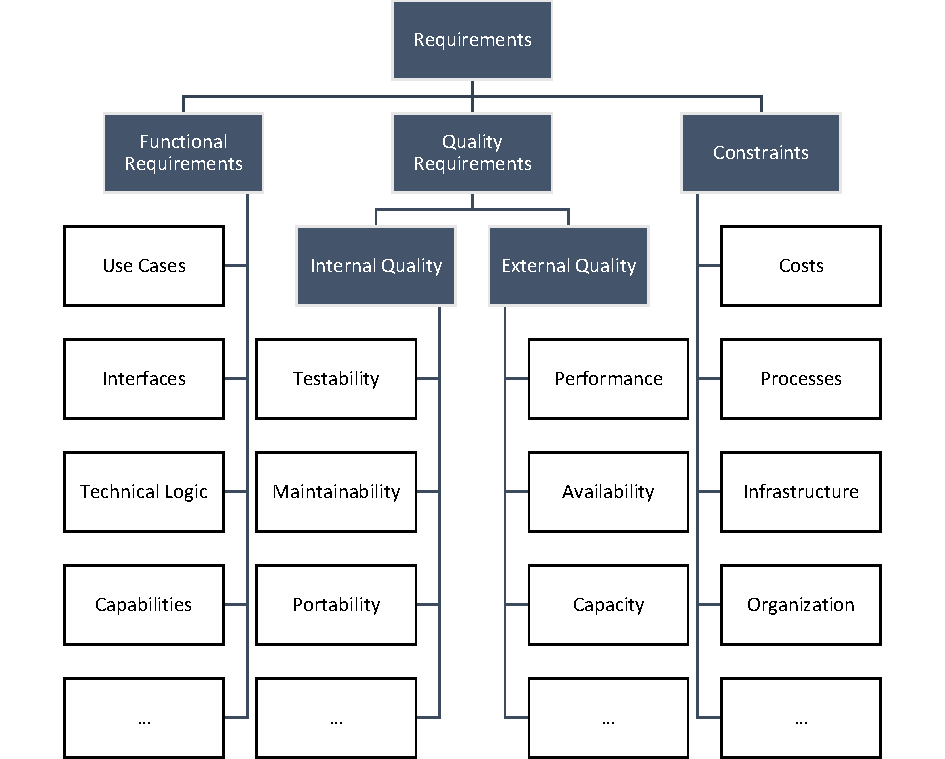
\includegraphics[scale=1]{img/RequirementTypes.pdf}
    \caption[Requirement Types]{Tpes of Requirements used in this paper (own illustration)}
    \label{fig:reqTypes}
\end{figure}
\subsection{Requirements Engineering}
\subsubsection{Motivation}
 
% TODO 
 
\subsubsection{Methodology \label{sec:methReq}}
Engineering requirements for a to-be system requires a diverse set of input information (cf. \Cref{fig:reqFlow}). The goal of Requirement Engineering is to produce a set of requirements fitting to a modeled and specified system \parencite[cf.][28]{Kotonya.2000}. A repetitive and systematic approach to generate complete, relevant, consistent etc. requirements is implied by Requirement Engineering \parencite[5]{Sommerville.2000}, including sourcing and management of requirements \parencite[262]{Pohl.2007}.
\begin{figure}[H]
    \centering
    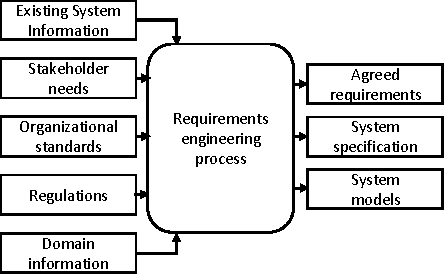
\includegraphics[scale=1.3]{img/RequirementInformationStream.pdf}
    \caption[Information flow in Requirements Engineering]{Information flow in Requirement Engineering (\protect\cite[28]{Kotonya.2000})}
    \label{fig:reqFlow}
\end{figure}
Information sources for Requirements Engineering include:
\begin{enumerate}
    \item Existing system information include all information about systems to be interacted with, as well as a potential legacy system \parencite[cf.][28]{Kotonya.2000}.
    \item Stakeholders of a system are people or institutions that have some kind of direct or indirect causal relation with the system \parencite[cf.][8]{Sommerville.2000}. This may be users, developers, sponsors, customers, employees and many more. Each stakeholder has some needs for the system - being motivated by political interests in the organization, support of work, legal determinations or something differently \parencites[cf.][28]{Kotonya.2000}[cf.][350-351]{Lauesen.2008}
    \item Organizational standards enforce conformaty assurance within one company by regulating system development, quality management etc. \parencite[28]{Kotonya.2000}
    \item Regulations seek to protect the interests of certain stakeholders, e.g. health and safety regulations \parencite[cf.][28]{Kotonya.2000}.
    \item \say{Domain information [..] about the application domain of the system} \parencite[28]{Kotonya.2000} 
\end{enumerate}

\paragraph{Requirement Engineering Process:} The\say{Requirements Engineering Framework} by \textcite{Pohl.2007} defines a systemic approach to fill the gap between input information and the vision and goals of a desired output (cf. \Cref{fig:reqFramework}). It analyzes the input information into four different facet of the system context: entities, IT-system, usage and development of the desired application. Information is processed in three main activities (documentation, sourcing and confirmation) and two cross-sectional activities (validation and management), which lead to the requirement artifacts which represent the vision and goals of the product. \parencite[cf.][38-39]{Pohl.2007}
\begin{figure}[H]
    \centering
    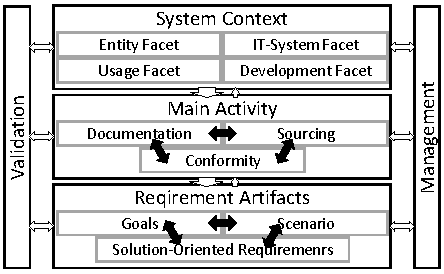
\includegraphics[scale=1.5]{img/ReqAnFrameWork.pdf}
    \caption[Framework for Requirements Engineering]{Framework for Requirements Engineering (own illustration based on \cite[41]{Pohl.2007})}
    \label{fig:reqFramework}
\end{figure}
\subparagraph{} Defining the boundary of system context is essential for successful requirements engineering. It reflects in what way the desired outcome is related entities of whatever kind \parencite[55]{Pohl.2007}. Context diagrams \parencites[cf.][266]{Kossiakoff.2011} - as an example for visual System Context representation - treat the system \say{as a black box surrounded by user groups and external systems with which it communicates} \parencite[76]{Lauesen.2008}. The System Context represents the environment of a system, which is relevant for requirement analysis \parencite[55]{Pohl.2007}. The boundaries of the system context must be defined to scope out the not relevant part of the environment \parencite[55-56]{Pohl.2007}. The four facets for structuring input information of the system context of \textcite{Pohl.2007} are the following:
\begin{enumerate}
    \item{Entity Facet} 
    Entities are the digital representation of real world objects and their traits. This can include people such as users and subjects, physical objects such as assets, immaterial objects such as measurements, and processes. Important stakeholders are  professionals for the technical view and legal advisor and data security officials ensuring compliance. \parencite[cf.][70-71]{Pohl.2007}
    \item The facet of the IT-system in the System Context is considering interface requirements to other technical systems such as the underlying hardware or systems the desired product must or may interchange data with \parencite[cf.][192]{Kotonya.2000}. Relevant stakeholders are architects, developers, and test and maintenance professionals of the context systems \parencite[cf.][72]{Pohl.2007}.
    \item The usage facet deals with the demand by direct and indirect users for the system. User in this context are people and systems having a direct interface with the desired product or are somehow impacting the interaction with the desired product or are impacted by usage of the system. \parencite[cf.][75-77]{Pohl.2007}
    \item All information about the development process is regarded by the development facet. Stakeholders and sources for this facet predominantly are people involved with the design, implementation and controlling of the development process, guidelines, standards and norms for development, and best practices and project reports. \parencite[cf.][79]{Pohl.2007}
\end{enumerate}

\begin{figure}[H]
    \centering
    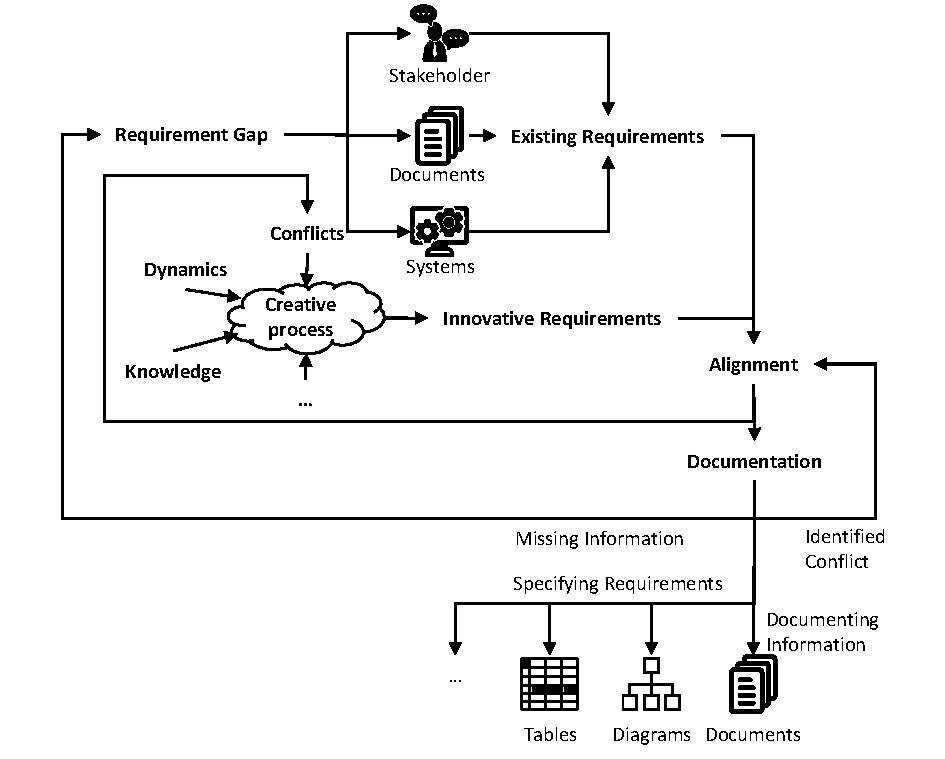
\includegraphics[scale=1]{img/MainActivity.pdf}
    \caption[Information Flow in Main Activity of Requirements Engineering]{Information Flow in Main Activity  (own illustration)}
    \label{fig:infFlow}
\end{figure}
\subparagraph{} The main activities are interlinked by continuously exchanging information. \Cref{fig:infFlow} sows a minimalist outline of that flow of information. Starting from the supplied information by stakeholders, documents, etc. requirements are generated, aligned for conformity, and specified and documented. Feedback loops resolve occurring errors such as conflicts of requirements or gaps.
\begin{enumerate}
    \item Sourcing requirements founds on two different goals: detecting existing requirements, and create innovative requirements \parencite[cf.][318, 321]{Pohl.2007}. This is done by taking information from the information sources (see \Cref{fig:reqFlow}) and analyzing the underlying needs \parencite[cf.][75-76]{Sommerville.2000}. Whenever conflicts of requirements, group dynamics etc. generate demand for an additional requirement without specific needs or a trade-off solution, a creative approach can be used to innovate new requirements \parencite[cf.][94]{Lauesen.2008}. 
    \item The conformity activity seeks and identifies competing requirements - in content, limited resources, or priority - in order to resolve those issues. The Conformity activity seeks to resolve those issues by analysis and management of conflicts. Possible solutions include management decisions, trade-offs, or inducing change requests. \parencite[cf.][393]{Pohl.2007}
    \item{Documentation} is used for recording all relevant information gathered in the main and cross-section activities \parencite[cf.][217]{Pohl.2007}. Requirements Engineering distinguish two subsets of documented information: documented requirements and specified requirements. Only requirements that have been parsed from informal descriptions - as they are most commonly provided by operational or marketing departments - into standardized requirement templates are specified requirements \parencite[cf.][101]{Ebert.2014}. Depending on the kind of information to be documented, different levels of specification are necessary. The documenting activity helps to identify gaps and conflicts in existing requirements giving input to the other main activities \parencite[212]{Pohl.2007}
\end{enumerate}

\subparagraph{} Requirement artifacts are documented requirements \parencite[85]{Pohl.2007}. There are three complementary categories of requirements: 

\begin{enumerate}
    \item Intentions of the stakeholders are documented as goals \parencite[cf.][85]{Pohl.2007}, substanciating the product vision \parencite[cf.][54]{Ebert.2014}. Goals are decomposed into groups of subgoals connected by logical AND and OR gateways \parencite[cf][91]{Pohl.2007}. Goal level requirements are optimal for understanding the reason for requirements, because they reflect the value of the requirement to the stakeholder \parencite[cf.][25]{Lauesen.2008}.
    \item Scenarios are list of steps in the system context that need to be done to fulfill a goal level requirement \parencite[125]{Pohl.2007}. \say{A scenario is an instantiation of a use case} \parencite[114]{Lauesen.2008}, meaning that each scenario matches a process within the system, or interaction with the system, including a desired outcome \parencite[cf.][114]{Lauesen.2008}.
    \item Deducing from goals and scenarios, solution-oriented requirements specify all relevant information for developing the desired application \parencite[cf.][182-184]{Pohl.2007}. These requirements are based on three different perspectives (data, functionality and behaviour) and are documented in natural language and/or in models \parencite[cf.][184-187]{Pohl.2007}. Commonly a sentence pattern is used for natural language documentation      
\end{enumerate}

\subparagraph{} Cross-Sectional Activities

\subsubsection{Implications}

\section{Visual Design}

The fisrt impression of an application is crucial. The credibility of a website is judged by users in less than 3.5 seconds, 75\% based on the aesthetics, among other factors \parencite[cf.][1]{Alsudani.2009}. In order to generate a graphical user interface (GUI) for the application, the psychological effects of perception must be taken into account.


\subsection{Psychology of Perception}

\paragraph*{} 
The Gestalt theory describes eight laws for aesthetic designs, in terms of using intuitive perceptions of human brains to visually group objects to create a visual composition \parencite[cf.][113]{Sternberg.2012}.

\begin{enumerate}
    \item \textbf{Law of Proximity:} Objects that are close to each other, are become associated (cf. \Cref{fig:prox}). For things to be relatively close to each other, groups must be separated by a larger white space \parencite{Seogaard.n.y.}.
    
    \item \textbf{Law of Similarity:} As to be seen in \Cref{fig:sim}, objects that share visual properties group themselves visually \parencite[cf.][2]{Bakar.2017}.
    
    \begin{figure}[H] 
        \begin{minipage}[b]{.5\linewidth}
            \centering
\includegraphics[width=0.94\textwidth]{img/proximity.pdf}
            \subcaption{proximity}\label{fig:prox}
        \end{minipage}%
        \begin{minipage}[b]{.5\linewidth}
            \centering
\includegraphics[width=0.94\textwidth]{img/similarity.pdf}
            \subcaption{similarity}\label{fig:sim}
        \end{minipage}
        \caption[Laws of Proximity and Similarity]{Examples of the laws of proximity and similarity (own illustrations)}\label{fig:law1}
    \end{figure}
    
    \item \textbf{Law of Symmetry:} Humans tend to perceive objects as two approximate symmetrical halves wherever possible; separate symmetric objects are therefore more likely to be perceived as being one coherent object \parencite[cf.][]{Soegaard.n.y.}.
    
    \item \textbf{Law of Closure:} Objects that are grouped by visual perception (e.g. by proximity or symmetry) are experienced as a whole (cf. \Cref{fig:clo}). This principle may suggest objects that are none-existent on the interface \parencite[cf.][]{Stevenson.n.y.}.
    
    \begin{figure}[H] 
        \begin{minipage}[b]{.5\linewidth}
            \centering
\includegraphics[width=0.94\textwidth]{img/symmetry.pdf}
            \subcaption{symmetry}\label{fig:sym}
        \end{minipage}
        \begin{minipage}[b]{.5\linewidth}
            \centering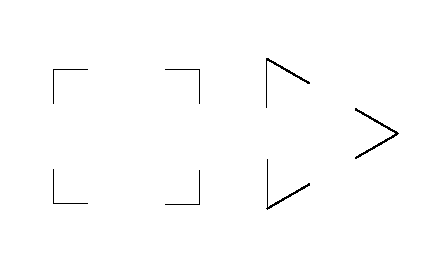
\includegraphics[width=0.94\textwidth]{img/closure.pdf}
            \subcaption{closure}\label{fig:clo}
        \end{minipage}%
        \caption[Laws of Closure and Symmetry]{Examples of the laws of closure and symmetry (own illustrations)}\label{fig:law2}
    \end{figure}
    
    \item \textbf{Law of Common Fate:} Objects that are moving in the same direction are visually connected, while separating those fixed in position or moving differently \parencite{Todorovic.2008}.
    
    \item \textbf{Law of Continuity:} Visual perception prefers to follow smooth lines. This may result in misleading predictions and a tendency to find smooth continuation more favorable than rough ones, but can also suggest users to follow a certain path of looking or navigating. \parencites{Bakar.2017}{Todorovic.2008}
    
    \begin{figure}[H] 
        \begin{minipage}[b]{.5\linewidth}
            \centering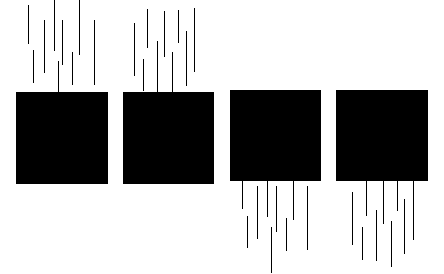
\includegraphics[width=0.94\textwidth]{img/fate.pdf}
            \subcaption{common fate}\label{fig:fate}
        \end{minipage}%
        \begin{minipage}[b]{.5\linewidth}
            \centering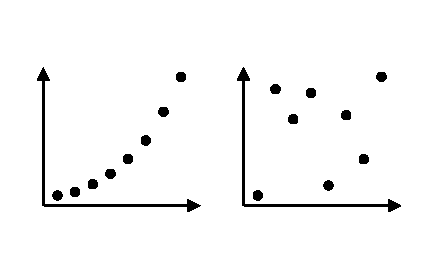
\includegraphics[width=0.94\textwidth]{img/continuity.pdf}
            \subcaption{continuity}\label{fig:con}
        \end{minipage}
        \caption[Laws of Common Fate and Continuity]{Examples of the laws of common fate and continuity (own illustrations)}\label{fig:law3}
    \end{figure}
    
    \item \textbf{Law of Good Gestalt:} Groups with regular patterns are more easily perceived and remembered than unstructured ones, because two different patterns within one group instinctively separate the group into two, as it can be seen in \Cref{fig:gest} \parencite{Todorovic.2008} on the right. 
    
    \item \textbf{Law of Past Experience:} Sometimes also called \textit{Law of Pragnance}, the law of past experience is the risk of a human to filter out information and reducing the perceived information to more common examples \parencite{Stevenson.n.y.}. In \Cref{fig:exo} an capital \say{L} and \say{I} will form a capital \say{U} in perception, which may not be the implicated goal. On the other hand one can use that profitable as the emoticon is a common way to express sentiment in short form.
    
    \begin{figure}[H] 
        \begin{minipage}[b]{.5\linewidth}
            \centering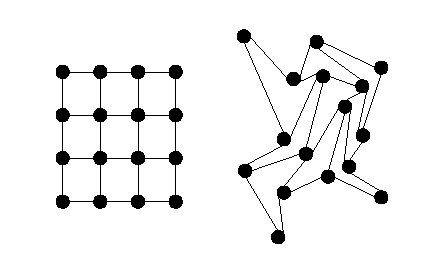
\includegraphics[width=0.94\textwidth]{img/gestalt.pdf}
            \subcaption{good gestalt}\label{fig:gest}
        \end{minipage}%
        \begin{minipage}[b]{.5\linewidth}
            \centering
\includegraphics[width=0.94\textwidth]{img/experience.pdf}
            \subcaption{past experience}\label{fig:exo}
        \end{minipage}
        \caption[Laws of Good Gestalt and Past Experience]{Examples of the laws of good gestalt and past experience (own illustrations)}\label{fig:law4}
    \end{figure}
\end{enumerate}


\subsection{Attention Economy \label{ssec:attention}}\label{beginAtt}
Attention economy deals with the scarcity of the ability of people to pay attention. In modern times, one does not only do one thing at work, but is continuously given information  \parencite[cf.][]{Davenport.2001}. \textcite{Davenport.2001} state, that for successful transfer of knowledge, understanding attention economy is essential. 

\paragraph*{} The attention of people is treated as a limited resource in the concept of attention economy. It is distinguished by the trait of being naturally limited and transient. This means, that a moment not used for paying attention for something may neither stored, nor restored \parencite[cf.][]{Davenport.2001}.

\paragraph*{} The reason for attention economy to become relevant is the increasing amount of available information. The increasing diversity and density of information is caused in the mainstream of digital media and the internet in form of online news, e-mail, social media etc. in addition to traditional communication and information channels such as TV, radio, telephony, letters etc.

\paragraph*{} Derived from the scarcity of attention, one can regard attention as a money worth good \parencite[cf.][]{Davenport.2001}. While market penetration is narrative for marketing purposes, one must take into account, that potential users of an application may leave it after a short period of time in favor of competing consumers of attention. Designing user interfaces to keep the user's attention, and winning it back later is key for conjoining the marketing idea and the implication of attention economy.\label{endAtt}
\section{Marketing}
In order to understand the special features of B2B marketing, in this chapter a fundamental overview of the marketing mix will be used to extract the relevant parts of marketing, that need to be considered for the conception of a application at it is desired. After showing the basic differences between B2B and consumer marketing, the impacts of these differences to the relevant part of the marketing mix will be described. In the end of this chapter the approach of market orientation for dealing with these specialties will be explained and described.
\subsection{Marketing Mix}
The term \textit{marketing mix} is be defined as the combination of different marketing instruments \parencite[cf.][285]{Thommen.2012}. There are  different categories of those instruments: originally described by \textcite[cf.][]{McCarthy.1993} the basic marketing mix, consisting of the so called \textit{4 Ps} "product, place, price, and promotion" \sekcite{McCarthy.1993}{}{Rafiq.1995}{}. This paper will use a more recent set of nomenclature, because it more precisely describes the contents of the categories. The recent naming maps place to \textit{distribution}, price to \textit{terms and conditions}, and promotion to \textit{communication}, while \textit{product} is not renamed \parencites[285]{Thommen.2012}[cf.][397-720]{Meffert.2015}. 
\paragraph*{} In addition to these points, even more recent approaches, also include the categories "participants [some times calles people; note from the author], physical evidence, and process" \parencite{Rafiq.1995}. \Cref{fig:aspects} shows all seven aspects.  and some examples for what they the individual categories including. This is not a complete list, but may help to minimize the likelihood of confusion. Beneath it, the categories are described with examples, and their link to the concept.

\begin{figure}[H]
	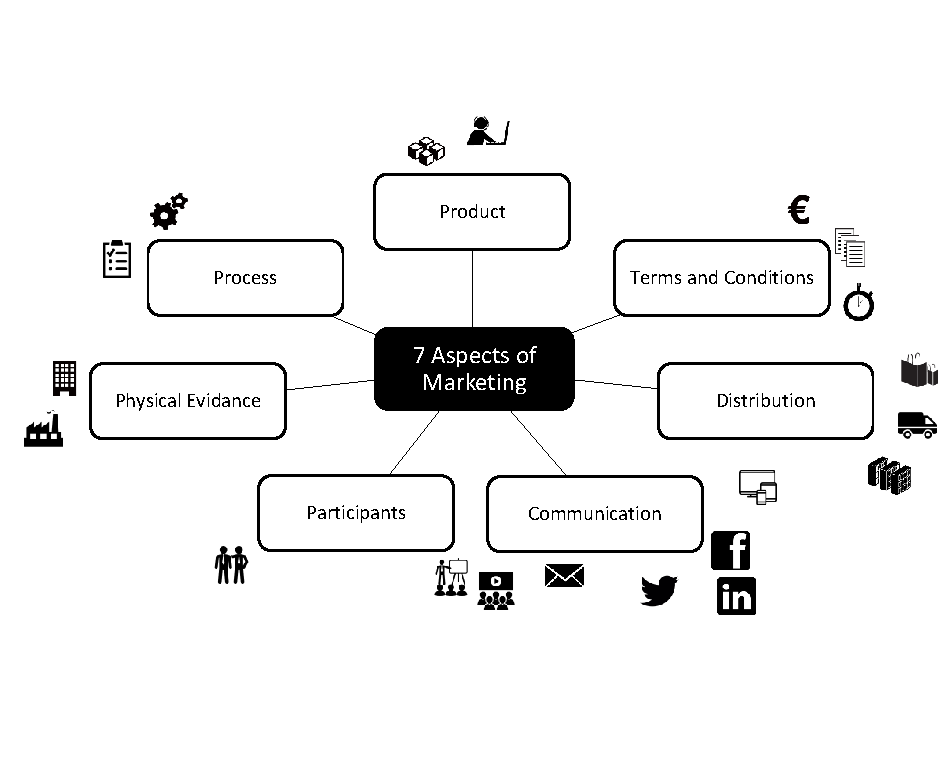
\includegraphics{img/7p.pdf}
	\caption[7 Aspects of Marketing]{The 7 Aspects of Marketing as used in this paper (own illustration based on \protect\cites[285]{Thommen.2012}[397-720]{Meffert.2015}{Hoepner2015})}
	\label{fig:aspects}
\end{figure}
\begin{enumerate}
    \item{Product:}The value of the individual product to be sold alone, and as part of the program of the selling company \parencite[cf.][398]{Meffert.2015}. As a example, the iPhone has certain features and specification. Additionally, it is part of the program of Apple, beside the iPad, several Mac Products and other things, including accessories and more. The individual product and its integration into the providers program can generate value to the customer, and different competitive advantages.
    \item{Terms and Conditions:}The terms and condition range from the price for purchase to service level agreements and warranty agreements, governing law, and many more. As an example, it is possible for several software products to be purchased with drastically different service levels tied to different prices. \\
    The contractual terms and conditions are negotiated by the customer and IBM for each case individually. Resulting from this, the desired application has no impact on this point, nor does it influence the desired instrument \parencite[cf.][]{Sachs.20.04.2017}.
    \item{Distribution:}The question of where and how you can purchase the product. For instance, it is possible to purchase the iPhone in a wide variety of stores, including Apple Stores, online, at most mobile service providers. On the other hand, the first One Plus was only available online and only by being invited by someone legitimate.\\
    The service sold, is by definition distributed as on-site, or remote service workers \parencite[cf.][]{Sachs.20.04.2017}. This as well cannot be influenced or changed by an pre-sales information application.
    \item{Communication:}This includes for example commercials, public relations, as well as sales men. \\
    The applications main goal is to build an additional channel of communication to the customer to explicitly show the technical competence of IBM. For that reason, the communication mix has a huge influence on the application, since it has to fit in an support other instruments of communication.
    \item{Participants:}The concrete individuals involved in placing the goods at the disposal. This includes for instance their skills and appearance. Someone dressed in a suit, may not be perceived as a creditable plumber. \\ 
    The participants of the service product can be different from each customer and project to the other. It may be possible to include information about the team in the application, which would underline the competence of each consultant.
    \item{Physical Evidence}
    \textcite[155]{AzilaGbettor2013} cite \textcite{Booms.1981} as describing the physical evidence, the physical environment surrounding the service. This explicitly targets the premises and related entities \parencite[cf.]{Hoepner2015}.
    \item{Process Parts:}
    The process parts describe the process of the contract fulfillment \parencite{Hoepner2015}.\\
    Thereby this has no direct influence on the pursed implementation. 
\end{enumerate}
\paragraph*{} As stated above, the outcome of this paper is connected to the communication, but as input for the design, the people and the product must be taken into account. 
\subsection{B2B versus B2C Marketing}
Several applications of the marketing instruments mentioned above are known from consumer market companies. Common examples PayPal's Terms and Conditions with their customer protection \parencite[see][]{PayPal}, the communication techniques of Apple etc.
\paragraph*{} \textcite[20-21]{Backhaus.2015b} states, that those consumer marketing and industrial marketing differ in several points.
\begin{table}[H]
\begin{center}
\begin{tabular}{|c|c|c|}
\hline 
 & Industrial Marketing & Consumer Marketing \\ 
\hline 
Demand & Derived & Direct \\ 
\hline 
Customers & Organizations & People \\ 
\hline 
Decision makers & Mainly multiple people & Mainly sole people \\ 
\hline 
Requirements & Formalized & Not formalized \\ 
\hline 
Market & Identified & Anonymous \\ 
\hline 
\end{tabular} 
\end{center}
\caption[Differences between industrial and consumer marketing]{Differences between industrial and consumer marketing (own illustration based on \protect\cite[21]{Backhaus.2015b})}
\label{tab:marketingdiff}
\end{table}
As to be seen in \Cref{tab:marketingdiff}, the circumstances for industrial - or B2B - marketing differ. It is worth taking a note, which points influence the conception of a marketing application as it is desired by this paper. 
\paragraph*{Demand:} The demand of a consumer market is by definition direct demand, since it is caused by a consumer wanting or needing something. The suppliers for the requested goods themselves require goods and services in order to fulfill the consumer needs. Therefore the B2B demand is derived from the direct demand \parencite[cf.][21]{Backhaus.2015b}. This implies, that one marketing strategy must be planned in respect to the downstream demand down to the consumer. 
\paragraph*{Customers:} Because organizations - not people - are the target customers in B2B marketing, the legal and organizational complexity must be considered, as explained in the following two points.
\paragraph*{Decision makers:}Regarding consumer purchases, the dominant part is decided on by an individual or a pair of two characters. Organizations on the other hand have larger groups of people involved in such a decision. This results in not only more people that have to be convinced, but also in differing target groups for the same product, e.g. the financial department, the technical department, and some operating department. 
\paragraph*{Requirements:}In consumer markets, suppliers try to anticipate the needs of the customers, and offer goods and services designed by these assumptions. In the B2B market this is still true for some products, in the specific field of this paper, customer companies define their requirements in their request for proposal. Therefore, it is possible to adapt the marketing mix to the individual case.
\paragraph*{Market:}In B2B markets, the supplier and customers are more likely to specifically know each other than in consumer good markets. For that reason, it id possible to identify needs in direct contact.
\paragraph*{} Those points can be linked directly linked to the point of communication. The benefits for communication in a B2B environment are  the direct contact between supplier and costumer, which generates the possibility for individualized communication approaches, and the formally described requirements, allowing direct referencing those. The downsides are larger decision groups are involved. They may be indirectly linked to the point of participants, since they are those in direct contact with the customer. They collect the lessons learned and formulate any technical information to be displayed in the desired application.
\paragraph*{}By the end of this section, all marketing related statements will relate to B2B marketing only.
\subsection{The Market Orientation Marketing Approach}
\textcite[9-10]{Claen.2016} shows that the term market orientation is used with a wide variety of definitions, from subjecting business to formulated customer demands only all the way to a complex orientation of business based on the complete market of the customer.
\begin{figure}[H]
	
\includegraphics[width=\textwidth]{img/supplychain.pdf}
	\caption[Supply Chain Schema]{Supply Chain Schema(own illustration based on \protect\cite{SouthwestTech})}
    	\label{fig:supplychain}
\end{figure}
The complete market in this context means the supply chain, as seen in \Cref{fig:supplychain}, and duties to all his stakeholders. \parencite[cf.][22-23]{Claen.2016}. A overview of the customers operational business at the center of his stakeholders, is sketched out in \Cref{fig:SGM}.
\begin{figure}[H]
	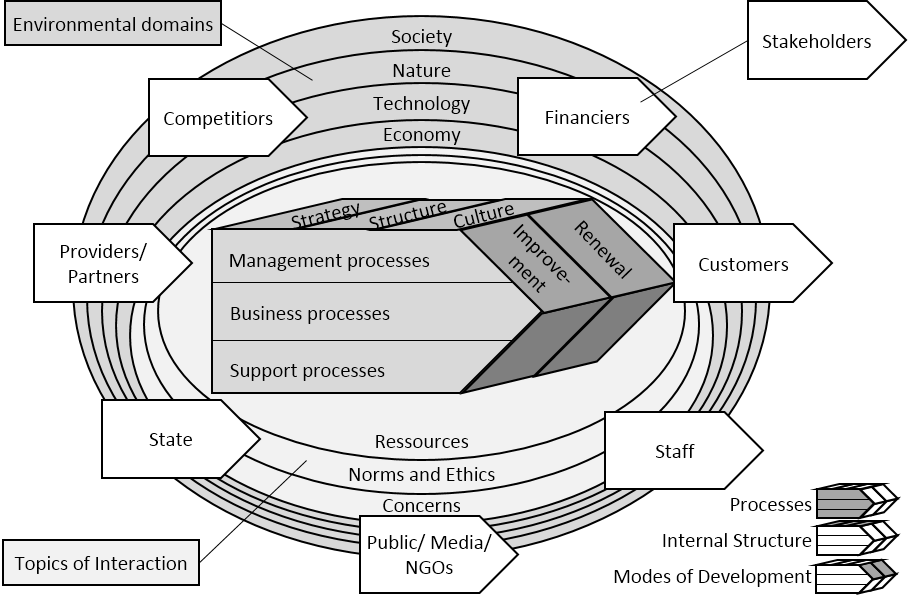
\includegraphics[width=1\textwidth]{img/SGM.png}
	\caption[St. Galler Management Modell]{The St. Galler Management Model from 2002 (own illustration based on \protect\cite{RueggSturm.2003})}
	\label{fig:SGM}
\end{figure}
The impact of this idea on the conception, which is the purpose of this paper, is that not only the direct customer of IBM and their decision makers must be analyzed for a sufficient planning of the application. The possible implication of the tendered project on the consumer and other stakeholder must become clear.

\chapter{Methodological Approach to Requirement Engineering}
\textcite[22-23]{Pohl.2007} explains, that applied requirements engineering always must be closely connected to the architectural planning of realization. This is because the architecture of a application induces insights, which can lead either to conflicts, or to gaps in the requirements set at the give state of work \parencites[22-23]{Pohl.2007} as displayed in \cref{fig:iterative}. 

\begin{figure}[H]
    \centering
    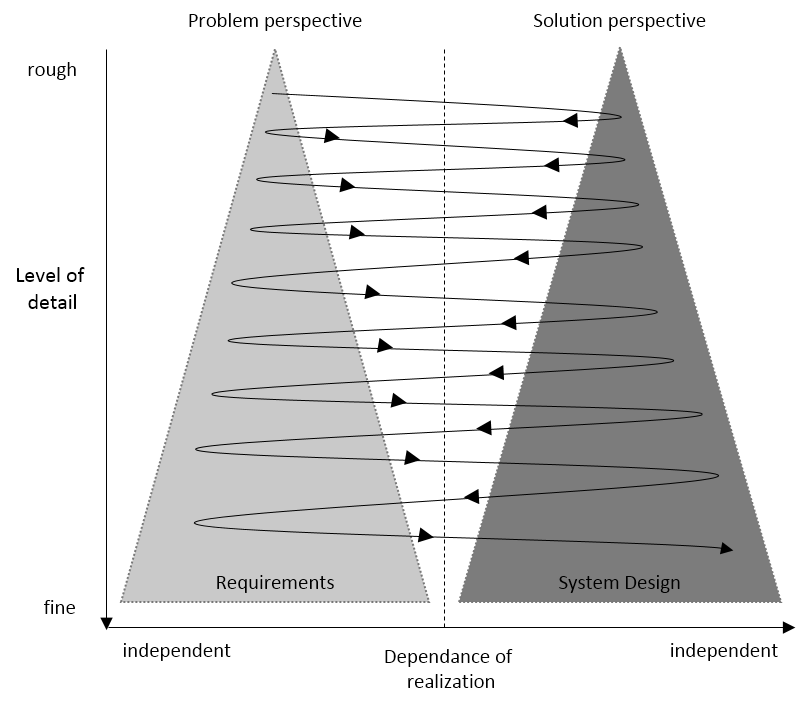
\includegraphics[width=0.7\textwidth]{img/iterative.png}
    \caption[Interdependence of Requirements and Design]{Interdependence of Requirements and Design \parencite[23]{Pohl.2007}}
    \label{fig:iterative}
\end{figure}

\paragraph{} This reflects the iterative nature of requirements engineering as described on \cpageref{iterative}. Thereby each step but the first of the following procedure will end in a check for bidirectional implications of architecture and requirement. The reason for the first step not following a checkup is, that no requirements are formulated yet. 


\paragraph{} This paper will begin with the definition of the context, and then perform the three main activities (cf. \cpageref{mainactivity} and \cpagerefrange{beginmain}{endmain}). In an iterative process, architectural designs will be done, as described above. 


\section{Finding the Context Definition}
This thesis will start the requirement engineering as suggested by \textcite{Pohl.2007} and described in \Cref{ssec:reqEn} by gathering information from the requirement sources. For orientation this paper will orientate at the source categories shown in \Cref{fig:reqFlow} on \cpageref{fig:reqFlow} going top down. 

\paragraph{} In the first instance, personas (see below) will be produced, in order to gasp the stakeholders. Withdrawing from the personas and other sources of information - some provided by the sponsor -, goals will be derived into use cases (see below). Those use cases will be analyzed for implications on the facets of the system context, as described on \cpagerefrange{beginFacets}{endFacet}. 


\subsection{Using Personas}
Human brains are caring more bout individuals, than large groups \parencite[cf.][]{Platt.2016}. Therefore, archetypal individual people \parencite[cf.][81-82]{Cooper.2007}, which embody specific characteristics of groups \parencite[cf.][]{Platt.2016} are more easy to gasp. That is the reason for using personas, which do exactly that.

\paragraph{} Identifying, analyzing, and prioritizing personas is a multistage procedure, which is always based on research \parencite[cf.][39]{Robier.2016}. Research methods for this kind do not claim to scientifically accurate, but must not be based solely upon stereotypes and arbitrary decisions \parencite[cf.][82-83]{Cooper.2007}. 

\begin{figure}[H]
\centering
    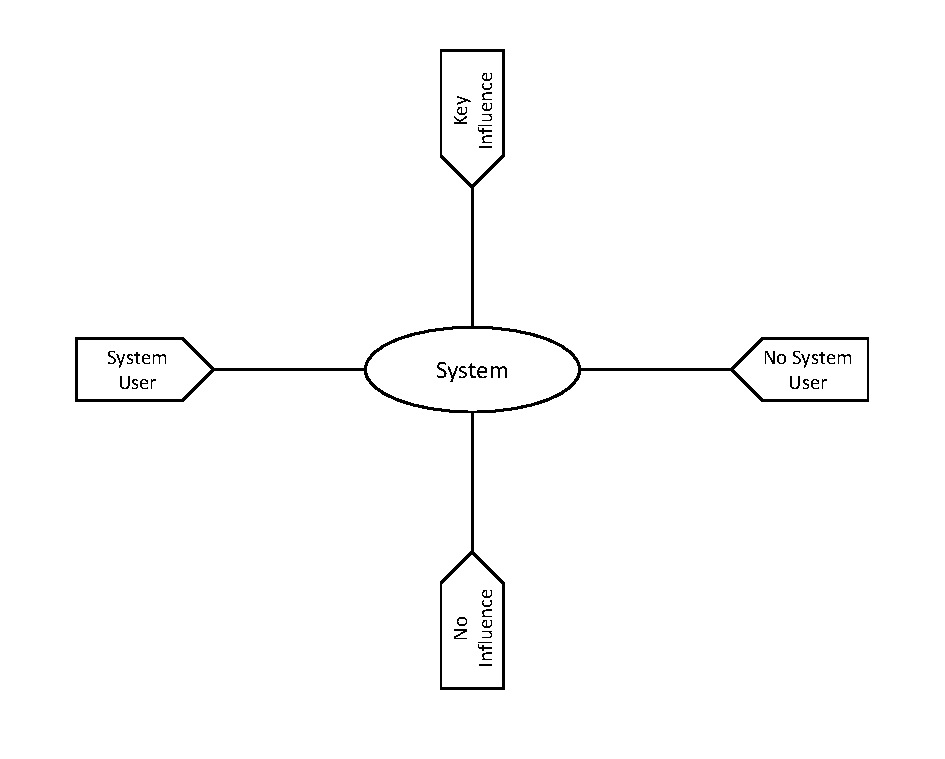
\includegraphics[scale=0.7]{img/stakeholderMap.pdf}
    \caption[Stakeholder Map]{Stakeholder Map (own illustration based on \cite[38]{Robier.2016})}
    \label{fig:stakeMap}
\end{figure}

\paragraph{} For identification of relevant stakeholders \textcite[38]{Robier.2016} suggest the usage of a stakeholder map (cf. \Cref{fig:stakeMap}). People of the left hand side of the vertical axis are the users of the program, divided into heavy users (far left) and fist time users (narrow to the axis) \parencite[cf.][38]{Robier.2016}.
\paragraph{} This approach aims not at the identification of each individual stakeholder, but at the identification of stakeholder groups to be represented by a persona \parencite[cf.][82]{Cooper.2007}, explicitly  including non-users \parencite[cf.][84]{Cooper.2007}.

\paragraph{} Analysis of the personas identified, includes the specification of a personas traits. Since personas are represented as individual people \parencite[cf.][81]{Cooper.2007}, it has all attributes a natural person has, including a name, gender, age, family, education, and most importantly: a motivation \parencites[cf.][]{Platt.2016}[cf.][83-84]{Cooper.2007}. All traits of a persona must be contributing to a bigger picture, and thereby must be intentionally be set to suggest intended characteristics \parencite[cf.]{Platt.2016}. 

\paragraph{} As an example: Our persona Kevin Smith (25, male) works at a international bank as foreign trade manager after his studies in financial management at Harvard Business School and needs a way to plan his meetings in accordance to required travel times. In his free time he has a private single engine plane. If you ask yourself whether Kevin needs his schedule in a standardized time zone, such as UTC, the answer will definitely be yes, because he is on the one hand used to using UTC at work and in his hobby. 

\paragraph{} Martha Jones (55, female) works at a local retailer since her diploma from community college, now being store manager, requiring a tool to plan and distribute shifts of her employees. She on the other hand will have more use for local time. Both may be personas for a calendar service focused on business customers. 

\paragraph{} All traits of Kevin and Martha will have implications on the conception and development of the hypothetical calendar service. Beside the very different functionality requests of transport service provider integration, respectively shift planning and public calendar provisioning, the age may have implications on the devices used, as well as the education implies different kinds of prior knowledge. 

\paragraph{} The prioritization of personas heavily depends on the specific product. It may be done by expected revenue (e.g. for sold services), least specialization (e.g. for training software) or any other reasonable technique for prioritization.

\begin{figure}[H]
    \centering
    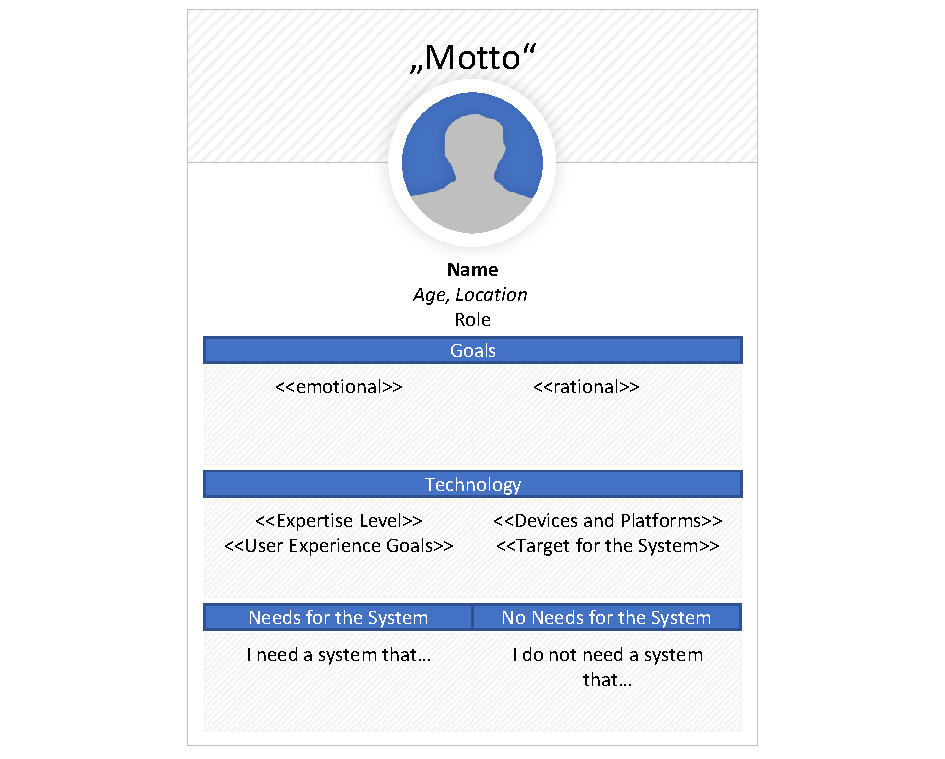
\includegraphics[scale=1]{img/PersonaTemplate.pdf}
    \caption[Template for Personas]{The template used for personas in this paper (own illustration)}
    \label{fig:persTemp}
\end{figure}

\paragraph{} The resulting personas are usually documented in a resume containing all relevant information \parencites[cf.][40]{Robier.2016}[cf.][]{Platt.2016}. This paper will use the template shown in \Cref{fig:persTemp}. It includes a picture of the persona, his or her personal information, his or her goals, needs, and for users his or her technological parameters.


\subsection{Using Use Case Diagrams}
\begin{figure}[H]
    \centering
    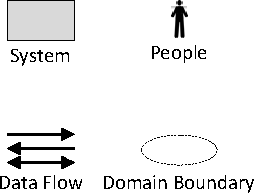
\includegraphics[scale=1]{img/SCDSymbols.pdf}
    \caption[Symbols of System Context Diagrams]{Symbols of System Context Diagrams \parencites[77]{Lauesen.2008}}
    \label{fig:scdSym}
\end{figure}
The system context diagram consists of four components: system, people, data flow, and domain boundaries \parencites[cf.][76-77]{Lauesen.2008}. Each one has its own representation, displayed in \Cref{fig:scdSym}. System context diagrams are used to identify required interfaces \parencites[cf.][75]{Lauesen.2008}, as well as to define the system boundary \parencites[cf.][75]{Ebert.2014}. It is an important overview of requirement sources, reflecting all interacting systems and persons. The direction of the arrow can show the direction of the data flow, or more commonly display the direction of intend \parencite[cf.][77]{Lauesen.2008}. In this paper the direction of an arrow will display the direction of intend.


\section{Main Activity}
\subsection{Sourcing Requirements from the Context}
The information of each facet will be compiled into goals for the desired outcome and which then will be clustered into the types of requirements described in \Cref{ssec:reqTypes} (cf. \Cref{fig:reqTypes} on \cpageref{fig:reqTypes}). The formulation of the goals will be done in a sentence stencil (see below) for requirement documentation. 

\paragraph{} The requirements will be itemized and clarified as much as possible to that point. Afterwards, the requirements will be prioritized and potential conflicts will be resolved. The reason for the prioritization before generating consistency is, that in case of an unreasonable conflict, the priorities must be clear to know which requirement to drop.


\subsection{Documenting the Requirements}
\subsubsection{In Natural Language}
Requirements must be expressed distinctly, in order to ensure the system is correctly developed \parencites[107]{Ebert.2014}. While natural language offers great possibilities, being universaly applicable, flexible and easy to use \parencite[cf.][239]{Pohl.2007}, there are some flaws regarding the distinctiveness. Languages have the troubles of containing  ambiguity, which are fatal for distinct communication \parencite[cf.][239-243]{Pohl.2007}.

\paragraph{}
\begin{figure}[H]
    \centering
    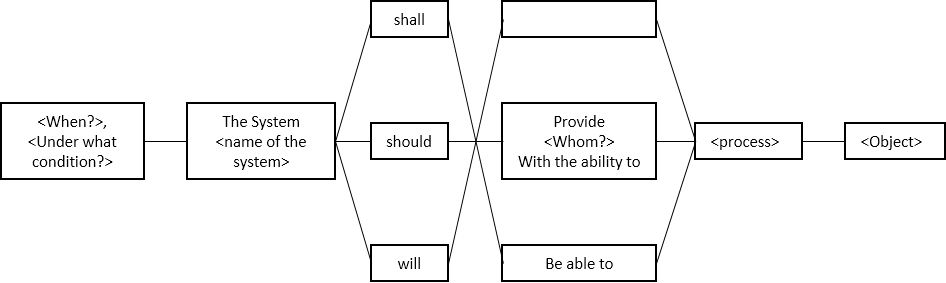
\includegraphics[width=\textwidth]{img/SentenceStructure.png}
    \caption{Requirement Documentation Sentence Structure (own illustration based on \cite[246]{Pohl.2007})}
    \label{fig:sentencestructure}
\end{figure}

\paragraph{} In order to counter these issues, this paper will use the sentence structure sugeested by \textcites[107]{Ebert.2014}[246]{Pohl.2007}. Sentence structures like these help to clarify and structure requirements, as log as only one requirement is represented per sentence \parencite[107]{Ebert.2014}. 


\subsubsection{In Diagram Notation}
For the diagram documentation of a requirement, a fitting diagram type must be selected \textcite[299]{Pohl.2007}.  This thesis will use use case diagrams for the documentation of goals of stakeholders. A use case diagram displays those by abstracting stakeholders into actors with goals when interacting with the system. Secondly, this paper will utilize sequence diagrams, which display the chronological set of interactions, as a tool to visualize scenarios. Last but not least, use cases and scenarios will be merged into function models, which display the flow of information in the complete system. 

\paragraph{} 
\begin{figure}[H]
    \centering
    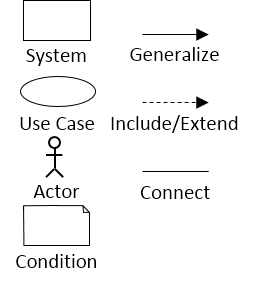
\includegraphics[scale=0.9]{img/ucSymb.png}
    \caption[Use Case Diagram Notation]{Use Case Diagram Notation (own illustration based on \cite[163]{Pohl.2007})}
    \label{fig:ucSymb}
\end{figure}
As mentioned above, use case diagrams consist actors, use cases and the system. It display in what kind the actors are directly or indirectly linked to the use cases. Both, actors and use cases, can be generalized in an aggregated version of themselves. The notation may be seen in \cref{fig:ucSymb}.

\begin{figure}[H]
    \centering
    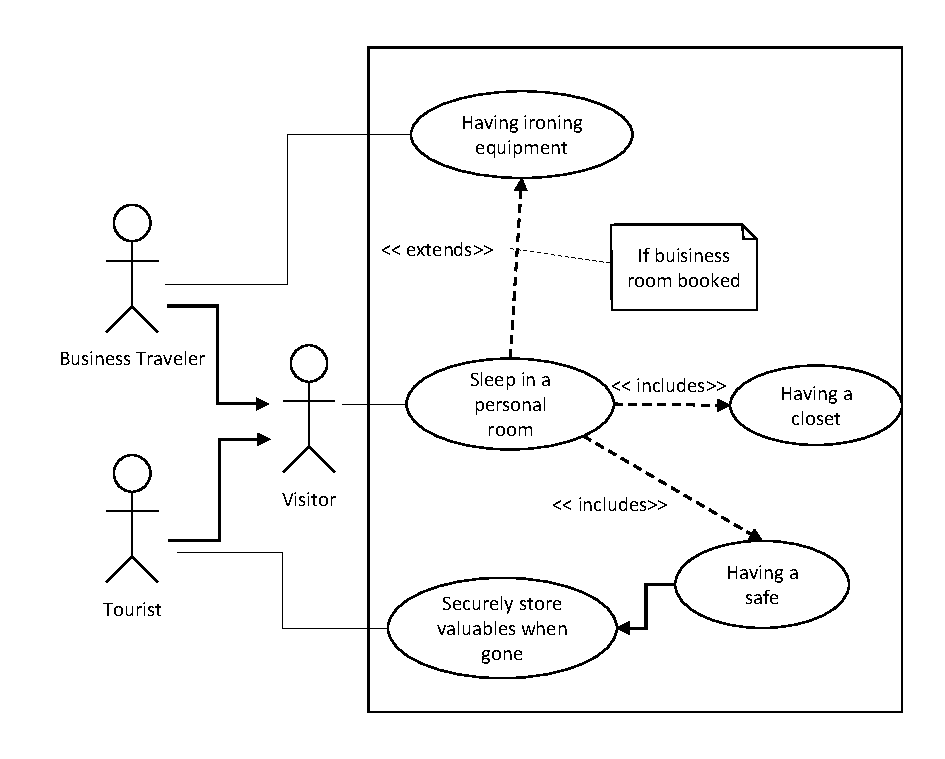
\includegraphics[scale=0.9]{img/ucEx.pdf}
    \caption[Example Use Case Diagram]{Use Case Diagram showing the Notation (own illustration)}
    \label{fig:ucEx}
\end{figure}

\paragraph{} As an example: business traveler and tourists are both visitors of hotels. They have different goals when visiting the hotel, but share some as well. The use case diagram will display the individual goals with the distinct actors, but generalize them to the visitor actor, which connects to the common goals. This example can be seen in \Cref{fig:ucEx}. 

\paragraph{} As seen in \Cref{fig:ucEx}, the goals do not have to be connected directly to the actor. They might be included in a different goal (e.g. the closet) or may extend other use cases under certain conditions (e.g. ironing eqippment).
 
\begin{figure}[H]
    \centering
    
\includegraphics[scale=0.9]{img/adSymb.png}
    \caption[Activity Diagram Notation]{Activity Diagram Notation (own illustration based on \cite[160]{Pohl.2007})}
    \label{fig:adSymb}
\end{figure}

\paragraph{} The activity diagram, on the other hand, expresses a chronological order of activities done by certain entities (system, user, etc.). Those diagrams have one start point and at least to end points, as well as activities, which are connected by control flow lines (cf.\cref{fig:adSymb}).

\begin{figure}
    \centering
    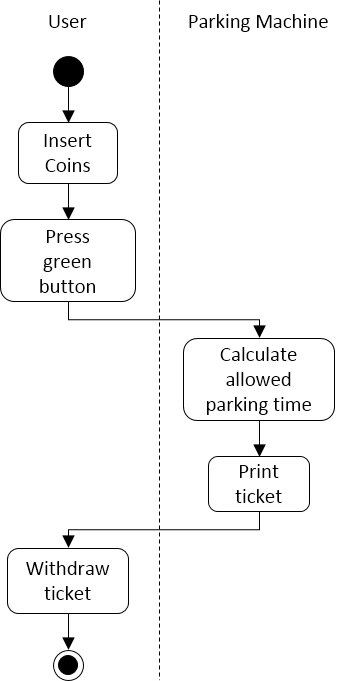
\includegraphics[scale=0.9]{img/activityDiagram.png}
    \caption[Example Activity Diagram]{Activity Diagram showing the Notation (own illustration)}
    \label{fig:adEx}
\end{figure}

\paragraph{} For demonstration \cref{fig:adEx} shows a activity diagram for a very simple parking ticket machine, as it is commonly used. What this demonstration leaks, is are logical gates such as AND or OR.

\paragraph{} 
\begin{figure}[H]
    \centering
    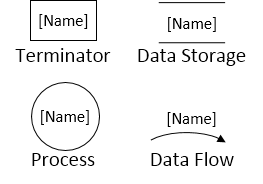
\includegraphics[width=0.5\textwidth]{img/fmSymb.png}
    \caption[Function Model Notation]{Function Model Notation (own illustration based on \cite[190]{Pohl.2007})}
    \label{fig:fmSymb}
\end{figure}


\subsection{Validating Conformity}
Scope Out

\section{Architectural Conception}
While the Unified Modeling Language (UML) \parencite[cf.]{}
\subsection{}


\section{User Interface Conception}


\subsection{Minimalist Approach of understandable User Interfaces}
Facing the challenges of \textit{Attention Economy}, business decision makers must explore applications at a higher speed that private users, because as stated above, spend attention implies costs of opportunity \parencite[cf.][]{Bakar.2017}. Therefore, designing a application must be done in optimization for fast knowledge transfer and easy exploration. In order to achieve this goal, \textcite{Bakar.2017} suggests a set of goals:
\begin{enumerate}
\item{Getting Started Fast} implies, that no unnecessary contents are disturbing the user from using the core functionality of the page by drastically removing  \say{explanatory and procedural information and let the user learn [...] through exploration} \parencite{Bakar.2017}.
\item{Training on Real Tasks} leads the user more easily receiving information and being more restrained by the application, due to a sense of excitement.
\item{Reading in Any Order} means the quality of the individual information to be not to have perquisite knowledge of any other page within the application.
\item{Exploiting Prior Knowledge} can help to keep the users attention by mostly presenting new information. This is documented as being dificult to be implemented successfully \sekcite{Carroll.1987}{}{Farkas.1990}{}.
\item{Coordinating System and Training} represents the progress of novice users in learning to work with the software. This is accomplished by keeping the users attention on the user interface and supplying constructive information.
\item{Supporting Error Recognition and Recovery} implies strong testing of the application to determine necessary error recognition and implement sufficient information recovery.
\item{Using the Situation} suggest providing the user many ways to explore the application in means of functionality and informational contents. Offering options for preoccupying oneself with the application amplifies the information transfer but increases the potential for errors.
\item{Developing Optimal Training Design} pertains the correlation of the user interface design to the users needs and behaviours. 
\item{Reasoning and Improvising} relatives the approach of explorative interaction by offering instructions where compulsory.
\end{enumerate}


\subsection{Outlining with Wire Frames}


\subsection{Prototyping with Mock-ups}

\newpage
\pagenumbering{Roman}
\addtocounter{savepage}{1}
\setcounter{page}{\thesavepage}

\defbibcheck{published}{%
    \iffieldundef{isbn}{%
        \iffieldundef{issn}{%
            \skipentry
        }{}%
    }{}%
}
\defbibcheck{online}{%
    \iffieldundef{isbn}{%
        \iffieldundef{issn}{%
            \iffieldundef{doi}{%
                \iffieldundef{url}{%
                    \skipentry%
                }{}%
            }{}%
        }{%
            \skipentry%
        }%
    }{%
        \skipentry%
    }%
}
\defbibcheck{gray}{%
    \iffieldundef{isbn}{%
        \iffieldundef{issn}{%
            \iffieldundef{doi}{%
                \iffieldundef{url}{}{%
                     \skipentry%
                }%
            }{%
                 \skipentry%
            }%
        }{%
             \skipentry%
        }%
    }{%
         \skipentry%
    }%
}

\defbibheading{bibliography}[\bibname]{%
    \section*{#1}%
    \markboth{#1}{#1}%
}
%\defbibfilter{online}{url and not isbn and not issn and not doi}
%\defbibfilter{other}{not url and not isbn and not issn and not doi}

\addcontentsline{toc}{chapter}{Bibliography}
\chapter*{Bibliography}
\addcontentsline{toc}{section}{Literature}
\printbibliography[check=published,title={Literature}]
\newpage
\addcontentsline{toc}{section}{Electronic Media}
\printbibliography[check=online,title={Electronic Media}]
\newpage
\addcontentsline{toc}{section}{Other Sources}
\printbibliography[check=gray,title={Other Sources}]
\chapter*{Appendix}
\addcontentsline{toc}{chapter}{Appendix}
%\renewcommand{\chaptermark}[1]{\markboth{}{\uppercase{#1}}}
\chaptermark{Appendix}
\begin{appendix}
\renewcommand\thechapter{\Alph{chapter}}
\section*{Appendix I}
\subsection*{Minutes form Memory I - Interview with an Expert}
Date: 20.04.2017
Place: Franfurt am Main
Duration: 13:00 to 14:00
Expert: Sachs, Markus
Interviewer: London, Nick
Topic: Condition for migration projects
\paragraph{How the projects are acquired:}
The customer decides for whatever reason, that it is necessary, or beneficial to migrate from their current banking software to another. Examples for this could be: a change of the software provider, outsourcing of the banks IT infrastructure, or the fusion of two bank, as well as a joint venture. The customer then sends out a request for proposal, on which companies can apply. After a first level of selection, some candidates are invited for a presentation day. The presentations have certain conditions, such as a set time frame. After the presentation day is over, the bank decides which applicant is selected for the order.
\paragraph{The challenges IBM faces during this procedure:}
IBM is often one of the more expensive providers. Additionally, many perceive the IBM as the hardware company it was in the last decade. They neither see the IBM as a software consulting, nor as a business consulting company.
\paragraph{Does IBM have done successful projects of this kind before?} Yes it has, but those cannot be named in this interview without permission of the customers. From these projects IBM employees have much experience with potential struggles coming up in this setting, plus the in depth knowledge of IBM regarding software and IT in general, IBM is well suited to find technical solutions for most known challenges. And since the purchase of PricewaterhouseCoopers' and lots of other business consulting companies, IBM is prepared to guide the customer in decisions, where technical solutions are not enough.


\end{appendix}

\end{document}
